\section{Evaluation}

\subsection{Detailed evaluation of examples}

Let us consider the following example:
$\alpha_1 = \{x_1 - x_2 \geq -4, -x_2 - x_3 \geq 5, 
  x_2 + x_6 \geq 4, x_2 + x_5 \geq -3\}; 
\beta_1 = \{-x_1 + x_3 \geq -2, -x_4 - x_6 \geq 0, -x_5 + x_4 \geq 0\}$. 
Our implementation produces the following trace:

\verbatiminput{../../Software/Cpp/OctagonsInterpolant/tests/traces/example1.txt}

The Z3 SMT solver provides mechanisms to modified the arithmetic engine 
and several plugins to specialize algorithm for specific theories. It contains a
proper specialization to work with Utvpi queries for satisfiability checking. However, 
       the interpolation APIs do not include mechanisms to specialize the 
       interpolation algorithm for Utvpi formulas. Thus, the interpolant obtained by Z3 
       for the above problem is : 
       (and ($\leq$ 9 (+ (* (- 1) x3) (* 2 x6) x1)) ($\leq$ (- 5) (+ (* (- 1) x3) (* 2 x5) x1))).
       We can notice by the coefficients in the result that the interpolant is not
       a Utvpi formula, thus Z3 must have reduced the problem to linear integer arithmetic.

  The result obtained by Mathsat is 
(and ($\leq$ (- 5) (+ x1 (+ (* (- 1) x3) (* 2 x5)))) ($\leq$ 9 (+ x1 (+ (* (- 1) x3) (* 2 x6))))) 
  which is the same as Z3 modulo the commutativity of the
  additions in the expression. Despite this difference, the following query 
  to Z3 verifies that the interpolation produced by our implementation implies 
  the interpolation produced by the SMT solver above mentioned; at the same time,
  the interpolant produced by the SMT solver does not imply our interpolant.

  \verbatiminput{../../Software/Cpp/OctagonsInterpolant/verification/example1_strongest_inter_verification.smt2}

  For the next example, let us consider $\alpha_2 = \{
  -x_2 - x_1 + 3 \geq 0, 
  x_1 + x_3 + 1 \geq 0, 
  -x_3 - x_4 - 6 \geq 0, 
  x_5 + x_4 + 1 \geq 0 
  \}; \beta_2 = \{
  x_2 + x_3 + 3 \geq 0,
  x_6 - x_5 - 1 \geq 0,
  x_4 - x_6 + 4 \geq 0
  \}$. Our implementation produces the following trace:

\verbatiminput{../../Software/Cpp/OctagonsInterpolant/tests/traces/example2.txt}

The interpolant obtained by Z3 is 
 (and ($\leq$ (- 4) (+ x3 (* (- 1) x2))) ($\leq$ (+ x3 x4) (- 6)) ($\geq$ (+ x4 x5) (- 1))); 
 and the interpolant produced by Mathsat is ($\leq$ (+ x2 (+ x3 (+ x4 (* (- 1) x5)))) (- 7)).
 Using Z3, we were able to verify that: 
 \begin{itemize}
 \item the interpolantion obtained by our implementation
 is equivalent to the interpolant obtained by Z3. 
 \item the interpolant obtained by our implementation implies the interpolant
 obtained by Mathsat, but the converse does not hold.
 \end{itemize}

\verbatiminput{../../Software/Cpp/OctagonsInterpolant/verification/example2_strongest_inter_verification.smt2}

\subsection{Performance comparison with iZ3 and MathSat}\label{performance_oct}

TODO: START change this
This discuss will discuss a parametrized problem which will allows to test 
our implementation and constrast the execution with other interpolant generation
algorithms from Z3 and MathSat.

\begin{lemma} \label{performance_test_lemma_oct}
  Let $x$ be a constant and $f$ an unary function in the EUF language. 
  For every $n \in \mathbb{N}$ the following conjunction is unsatisfiable:
  \begin{equation*}
    f^n(x) = f^{n+1}(x), f^2(x) = x, f(x) \neq x
  \end{equation*}
  where $f^n(x)$ denotes de application of the function $f$ n-times
  to the constant $x$.
\end{lemma}

\begin{proof}
  Applying the congruence and transitive rules to the equation $f^2(x) = x$, 
  we can prove that for any number $n$ the two following equations hold:
  $x = f^{2n}(x)$ and $f(x) = f^{2n+1}(x)$.

  At this point we distinguish two cases for $n$:

  \begin{itemize}
    \item Case $n$ is even: Then $\exists m \in \mathbb{N} . n = 2m$.
      So by choosing $n = m$ to the above sequence
      and by the axiom $f^{2m}(x) = f^{2m+1}(x)$ we have that
      $x = f(x)$.
    \item Case $n$ is odd: Similarly to the previous reasoning, 
      we can also infer the equation $f^{2m+1}(x) = f^{2m+2}(x)$
      by congruence, so $x = f(x)$.
    \end{itemize}

    In both cases the equation $x = f(x)$ reaches contradiction with the
    disequality $x \neq f(x)$.
\end{proof}

The interpolation pair for our performance test 
is $(f^n(x) = f^{n+1}(x) \land f^2(x) = x \land f(a) \neq a, x = a)$
for fixed $n \in \mathbb{N}$.
It is easy to see that the pair is inconsistent due to the lemma 
\ref{performance_test_lemma_oct}. 

By lemma \ref{performance_test_lemma_oct}
we can also see that the formula $x = a \rightarrow \bot$ is an 
interpolating formula for all fixed $n$ in this parametrized problem.
We designed this problem because it is easy to verify the 
correctness of output of the algorithms and to measure 
the time used by the algorithms for large values of $n$. 
We executed instances of this problem for values of $n$
in the range $\{1, \dots, 10000\}$ using a computer desktop
equipped with an Intel i7-9700 @ 4.70 GHz and 16Gb of memory. 
The output produced by the interpolant generation algorithms
were the expected formula.
The following graphs reports the time measured by the UNIX
utility $times$ of our implementation, iZ3, and the interpolation 
generation algorithm from Mathsat.

TODO: END change this

\begin{figure}
  \centering
  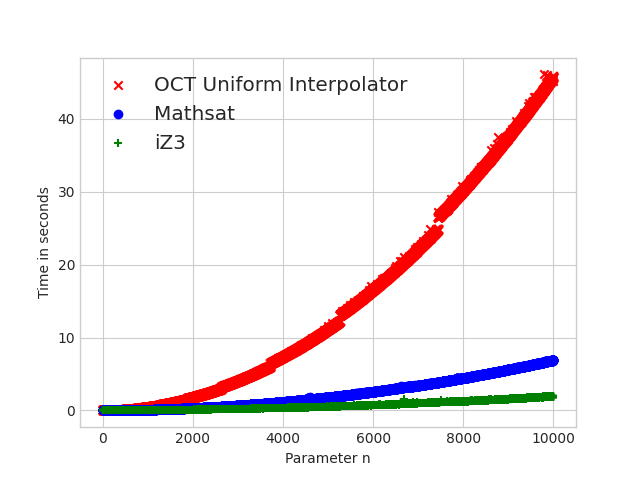
\includegraphics[scale=0.9]{figures/octi_performance_graph}
  \caption{Performance comparison graph of Oct interpolant generation
  algorithms for paramatrized problem from section \ref{performance_oct}} 
  \label{performance_graph_euf}
\end{figure}

TODO: change the following
We noticed a quadractic behaviour in the graph for the time 
required by our implementation
and a linear behaviour by iZ3 and Mathsat. However, 
according to the following polynomial 
fitting computation, 
we noticed that for the case of our implementation, 
a linear fitting obtained a smaller 
quadratic error compared to the quadratic fitting;  
for the case of the Mathsat
results, a quadratic fitting obtained a smaller 
quadratic errror.

\begin{table}[h]
  \centering
  \begin{tabular}{ccc}
    \toprule
    {}                 & Error of linear fitting & Error of quadratic fitting \\
    \cmidrule{2-2} \cmidrule{3-3} \\
    iZ3                & 3.2311742677852644e-25 & 1.269128969536517e-23       \\
    Mathsat            & 2.3207586060940883e-22 & 1.1983240884566356e-22      \\
    Our implementation & 2.9778502051908996e-21 & 1.455131710005814e-20       \\
    \bottomrule
  \end{tabular}
  \caption{Table of polynomial fitting errors of degrees 1, 2 for the
  Octagon experiments of section \ref{performance_oct}.}
\end{table}

%%% Local Variables:
%%% mode: latex
%%% TeX-master: "main"
%%% End:
